\documentclass[12pt]{article}
\usepackage{hyperref}
\usepackage{listings}
\usepackage{biblatex}
\usepackage{tikz}
\usepackage{refstyle}
\usepackage{mathabx}
%\usepackage{amssymb}
\usepackage{caption}
\usepackage{float}
\usepackage{graphicx}
\usepackage{graphics}
\usepackage{subfig}
\providecommand{\mbf}{\mathbf}
\providecommand{\pr}[1]{\ensuremath{\Pr\left(#1\right)}}
\providecommand{\re}[1]{\ensuremath{\text{Re}\left(#1\right)}}
\providecommand{\im}[1]{\ensuremath{\text{Im}\left(#1\right)}}
\providecommand{\qfunc}[1]{\ensuremath{Q\left(#1\right)}}
\providecommand{\sbrak}[1]{\ensuremath{{}\left[#1\right]}}
\providecommand{\lsbrak}[1]{\ensuremath{{}\left[#1\right.}}
\providecommand{\rsbrak}[1]{\ensuremath{{}\left.#1\right]}}
\providecommand{\brak}[1]{\ensuremath{\left(#1\right)}}
\providecommand{\lbrak}[1]{\ensuremath{\left(#1\right.}}
\providecommand{\rbrak}[1]{\ensuremath{\left.#1\right)}}
\providecommand{\cbrak}[1]{\ensuremath{\left\{#1\right\}}}
\providecommand{\lcbrak}[1]{\ensuremath{\left\{#1\right.}}
\providecommand{\rcbrak}[1]{\ensuremath{\left.#1\right\}}}

\graphicspath{{/storage/self/primary/Download/latexnew/fig}}
\begin{document}
\title{\textbf{ASSEMBLY}}
\date{}
\maketitle
\begin{enumerate}
   % \item \textbf{Question(GATE-EC-2018-46):}Given below \figref{fig:1} is the diagram of a synchronous sequential circuit with one $J-K$ flip-flop and one $T$ flip-flop with their outputs denoted as A and B respectively,with$J_A = (A'+B'),K_A = (A+B)$,and $T_B = A.$
   \item  \textbf{Question(GATE-EC-2018-46):}In the circuit shown below, a positive edge-triggered D Flip-Flop is used for sampling input
data $D_{in}$ using clock $CK$. The XOR gate outputs 3.3 volts for logic HIGH and 0 volts for logic LOW levels. The data bit and clock periods are equal and the value of $\Delta{T}/{T_{CK}}=0.15.$
where the parameters $\Delta{T}$ and $ T_{CK}$are shown in the figure. Assume that the Flip-Flop and the
$XOR$ gate are ideal.

 \begin{figure}[!h]
        \centering
        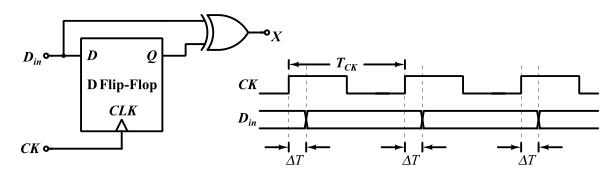
\includegraphics[width=\columnwidth]{figs/2018-gate-ec-46.png}
        \caption{}
        \label{fig:2018-gate-ec-46}
    \end{figure}

   
   % Starting from the initial state $(AB=00)$,the sequence of states $(AB)$ visited by the circuit is
   If the probability of input data bit $( D_{in} )$ transition in each clock period is $0.3$, the average
value (in volts, accurate to two decimal places) of the voltage at node $X$, is \dots



\end{enumerate}


\end{document}
